%
% Body text font is Palatino!
%

\documentclass[a5paper,pagesize,10pt,bibliography=totoc,numbers=noenddot,
headings=normal,DIV=9,twoside=false]{scrbook}

% twoside, openright
\KOMAoptions{DIV=last}

\usepackage{trajan}
 
\usepackage[french]{babel}
%\usepackage[utf8]{inputenc}
\usepackage[T1]{fontenc}
\usepackage[protrusion=true]{microtype}
\usepackage[babel]{csquotes}
% Désactive l'étiquette de la figure dans les légendes
\usepackage[labelformat=empty]{caption}
\usepackage{hyperref}
\usepackage{tabularx}

\usepackage[sc]{mathpazo}
\linespread{1.05} 

\usepackage{xspace}

% Indentation des paragraphes
\setlength{\parindent}{10pt}
% Sauts de ligne entre les paragraphes
\setlength{\parskip}{1.4ex plus 0.35ex minus 0.3ex}
%\setlength{\parskip}{1.4ex plus 0.35ex minus 0.3ex}

% Pas de numérotation au-delà des chapitres
\setcounter{secnumdepth}{\chapternumdepth}

\title{A book title}   
\author{Author Name} 
\date{\today} 

\begin{document}


%=========================================
\begin{titlepage}
		\centering{
			{\fontsize{40}{48}\selectfont 
			A book title}
		}\\
			
		\vspace{10mm}
		\centering{\Large{Author Name}}\\
		\vspace{\fill}
		\centering \large{2011}
\end{titlepage}


%=========================================
\newpage{}
\thispagestyle {empty}

\vspace*{2cm}

\begin{center}
	\Large{\parbox{10cm}{
		\begin{raggedright}
		{\Large 
			\textit{Do what you think is interesting, 
			do something that you think is fun and worthwhile, 
			because otherwise you won’t do it well anyway.}
		}
	
		\vspace{.5cm}\hfill{---Brian W. Kernighan}
		\end{raggedright}
	}
}
\end{center}

\newcommand\keywords[3]{%
	\section*{Mots-clés :}

	\textbf{Cadre} : #1

	\textbf{Genre} : #2

	\textbf{Thème} : #3
}%

\newcommand\medfan[1]{%
	\emph{medfan}
}%

\newpage


%=========================================
\chapter*{Préambule}

Cet ouvrage est un ensemble de 31 scénarios hétéroclites conçus pour être joués dans des jeux de rôle sur table.
La plupart de ces histoires sont volontairement ouvertes, laissant aux joueurs et joueuses le soin de combler les vides et de préciser les flous par leur imagination.
Grâce à cette liberté d'interprétation, les scénarios ne sont attachés ni à des systèmes spécifiques, ni à des univers particuliers.
Les différentes aventures font donc la part belle à l'improvisation.

Chaque scénario est décrit par trois mots-clés :
\begin{itemize}
	\item le cadre dans lequel il a été imaginé,
	\item le genre d'histoire racontée,
	\item le thème de l'aventure.
\end{itemize}

Un index en fin d'ouvrage permet de retrouver la liste des scénarios relevant des différents mots-clés.
Ceux-ci sont toutefois à prendre comme des indications et non des obligations.
La plupart des aventures peuvent aisément être transposées d'un cadre à un autre voire d'un genre à un autre.

Les scénarios sont divisés en trois sous-parties: l'accroche, les péripéties et la résolution.
L'accroche, plus ou moins longue, pose la situation initiale dans laquelle se trouvent les personnages.
Les péripéties forment le gros de l'aventure et contient les éléments d'histoire à découvrir et les rebondissements du scénario.
Enfin, la résolution donne quelques pistes sur les façons de conclure l'aventure.

Les protagonistes des différentes histoires ne sont généralement pas nommés pour vous permettre d'y insérer les personnages de votre choix.
Toutefois, à chaque scénario est associé une fiche de personnage en deux lignes décrivant le caractère, les forces et les faiblesses d'un personnage non-joueur de l'aventure.
À vous de choisir si vous utilisez ces informations, elles ne sont là que pour faciliter la préparation du scénario!

Bonne lecture!

\chapter{L'anneau gardien}
\keywords{\medfan}{Aventure}{Objet magique, malédiction, altruisme}

\section{Scénario}

Ce scénario peut être facilement joué en parallèle d'une campagne \emph{medfan}, il suffit qu'un personnage obtienne l'anneau du titre.
C'est encore mieux si les joueurs l'utilisent régulièrement de leur propre chef.

La guerrière peut être remplacée par n'importe quelle figure combattante du moment qu'elle est suffisamment puissante pour servir d'ange gardien.

\subsection*{Accroche}

Les personnages entrent en possession d'un anneau magique.

\subsection*{Péripéties}

À chaque fois que la personne qui porte l'anneau est en danger de mort, une puissante guerrière se matérialise à proximité pour la tirer de ce mauvais pas.
Une fois le porteur en sécurité, la guerrière disparaît sans un mot et se contente de jeter un regard furieux en direction du groupe.

Chaque invocation semble l'énerver encore plus mais tout effort de lui parler est vain: elle ne parle pas et ne semble de toute façon pas les comprendre.

Au fil du temps, certaines de ses apparitions deviennent étranges. Parfois, la guerrière apparaît sans armes ni armures.
Une fois, elle se matérialise même un morceau de poulet à la main.

Un jour, elle finit par se matérialiser, tenant un morceau de papier à la main écrit dans une langue étrangère.
Après l'avoir déchiffré, le message dit ceci:
\blockquote{L'anneau est maudit. J'ai une famille et une vie. Je n'ai pas demandé à servir d'ange gardien. Le forgeron qui l'a créé est prisonnier des geôles royales. Trouvez-le et faites-lui lever la malédiction. S'il vous plaît.}


\textbf{Explications}: le forgeron est un sorcier malchanceux fuyant la guerre qui ravage une nation voisine.
Craignant pour sa vie, il a embauché des mercenaires pour l'escorter jusqu'au royaume des personnages mais alors que l'argent est venu à manquer, il s'est retrouvé sans aucune protection.
Pour assurer ses arrières, il n'a alors rien trouvé de mieux pour assurer sa sécurité que de lier l'âme d'une grande aventurière à la retraite -- croisée au hasard de son voyage -- à son anneau.

Une fois arrivé, le sorcier-forgeron a posé ses valises dans la capitale et s'y est établi comme fabriquant d'objets magiques.
Malheureusement, n'étant pas un bon gestionnaire, il s'est rapidement retrouvé criblé de dettes auprès du royaume, incapable d'honorer les commandes du gouvernement.
La milice l'a alors mis en prison avant de piller son échoppe et de vendre ses biens aux enchères pour rembourser ses dettes.
De fil en aiguille, l'anneau a ainsi échappé à son propriétaire et la guerrière subit tant bien que mal les aventures de son porteur, régulièrement importunée par ces invocations involontaires.

\subsection*{Résolution}

Plusieurs façons de lever le sortilège sont envisageables.
Si les personnages sont versés en magie, peut-être qu'un rituel impliquant la guerrière en personne pourrait briser le lien entre elle et l'anneau.
Ou bien peut-être qu'il suffirait de substituer une nouvelle âme pour libérer celle qui se trouve actuellement liée.
Enfin, en retrouvant la trace du sorcier, celui serait sûrement prêt à annuler son sort si on le sort des geôles, en payant ses dettes\dots ou bien par la force.

\chapter{L'incident du peuplier}
\keywords{Contemporain}{Action}{Militaire, diplomatie, guerre froide}

\section{Scénario}

Ce scénario est inspiré d'un fait réel ayant eu lieu en août 1976 (le \emph{poplar tree incident})\footnote{\url{https://fr.wikipedia.org/wiki/Incident_du_peuplier}} dans la zone démilitarisée (DMZ) séparant la Corée du Nord de la Corée du Sud.
Comme beaucoup d'autres incidents diplomatiques de l'époque, la tension découle en grande partie du contexte de guerre froide entre deux superpuissances.

\subsection{Accroche}

Août 1976. Zone démilitarisée coréenne, section contrôlée par l'ONU. Un groupe de soldats coréens et américains s'apprête à tailler les branches d'un peuplier car celles-ci masquent leur ligne de vue sur le \og pont de Non-retour\fg.
Ledit pont est l'unique passage permettant aux nord-coréens de traverser la rivière Sachon pour rejoindre leur propre zone.
Quinze minutes plus tard, un camion de soldats nords-coréens arrive.
Ils demandent aux onusiens de stopper l'élagage de l'arbre car celui-ci aurait été planté par Kim Il-sung en personne.
Devant leur refus, ils attaquent le contingent à coups de hachettes et de gourdins, tuant deux officiers américains et capturant plusieurs soldats.

\subsection{Péripéties}

L'incident enflamme la zone.
Les nord-coréens dénoncent une agression américaine et reçoivent le soutien immédiat de Cuba et de nombreux pays non-alignés.
En face, la CIA considère que l'attaque nord-coréenne était préméditée et les États-Unis passent en DEFCON3.

Les commandement de l'ONU ou l'état-major des États-Unis mobilise les personnages dans le cadre de l'opération \emph{Paul Bunyan}, du nom de légendaire bûcheron américain.

Des sapeurs du corps d'ingiénerie de l'armée de terre sont diligentés pour abattre l'arbre.
Un bataillon de soldats américains est envoyé comme escorte, épaulé par les forces spéciales coréennes.
En appui de cette démonstration de force, plusieurs hélicoptères et avions de combat sont déployés dans l'espoir d'intimider le régime nord-coréen.
Les forces armées pénètrent ainsi dans la DMZ et l'impressionnante armada converge vers le peuplier à deux pas du pont de non-retour.
Très rapidement, plusieurs bus militaires nord-coréens arrivent sur site pour préparer la riposte.
Des soldats en descendent et déploient des mitrailleuses sur l'autre rive.

L'objectif de l'opération \emph{Paul Bunyan} est simple: abattre le peuplier tout en évitant la guerre.

Le tableau de la page \pageref{table:peuplier} comporte quelques événements aléatoires permettant d'épicer la situation et de maintenir les joueuses sur le qui-vive.

\subsection{Résolution}

En fonction des décisions du groupe et de leurs réactions aux événements, le conflit peut très facilement être désamorcé (après tout, l'équilibre des forces est très en défaveur des nords-coréens).
Même une escarmouche ou une fusillade, si elle est maintenue sous contrôle, ne risque pas de dégénérer en une guerre ouverte.
Cependant, la violence peut vite prendre de l'ampleur si personne ne s'en préoccupe.
L'idée est de mettre de scène une escalade lente mais inéluctable de l'opposition entre les deux factions et de jouer sur la tension qui l'accompagne.
Il ne faut donc pas hésiter à rendre les choses difficiles pour les personnages: rien ne doit se passer comme prévu et chaque petite erreur ou entorse aux consignes a le potentiel d'être l'étincelle qui met le feu aux poudres.

\begin{table}
	\caption{Événements aléatoires durant l'abattage du peuplier}
	\label{table:peuplier}
	\colortablerows
	\begin{tabularx}{0.9\textwidth}{cX}
	d8 & Événement\\
	1  & Les tronçonneuses tombent en panne après quelques minutes. Il faut soit en faire venir des nouvelles, soit finir le travail à la hache.\\
	2  & Un soldat américain s'avance sur le pont et provoque les nord-coréens. Il se trouve qu'il est proche d'un des officiers assassinés.\\
	3  & Des camions nord-coréens s'installent à 150m\dots et construisent un nouveau pont.\\
	4  & Les nord-coréens font s'avancer les prisonniers sur le pont. Ils seront relâchés si les forces impérialistes renoncent, sinon ils seront exécutés.\\
	5  & Un des soldats sud-coréens se comporte étrangement. Il transmet discrètement des informations au régime du nord sur l'avancée de l'opération américaine.\\
	6  & Les renseignements japonais ont intercepté un message nord-coréens : leurs troupes s'apprêteraient à bloquer la rivière Imjin. C'est malheureusement la route prévue par le commandement de l'ONU pour une évacuation par canots en cas d'attaque\dots\\
	7  & Un jeune nord-coréen saute dans la rivière et tente de traverser à la nage. Il appelle à l'aide en anglais et jure qu'il veut faire défection.\\
	8  & Alors que les sapeurs ramassent les branches déjà coupées et les chargent dans un pick-up conformément aux ordres, les sud-coréens leur demandent de les laisser sur place. Compte-tenu du symbolisme de l'arbre, les nords-coréens pourraient prendre cet acte pour une provocation.\\
	\end{tabularx}
\end{table}

\subsection*{Lieu: la zone jointe de sécurité}

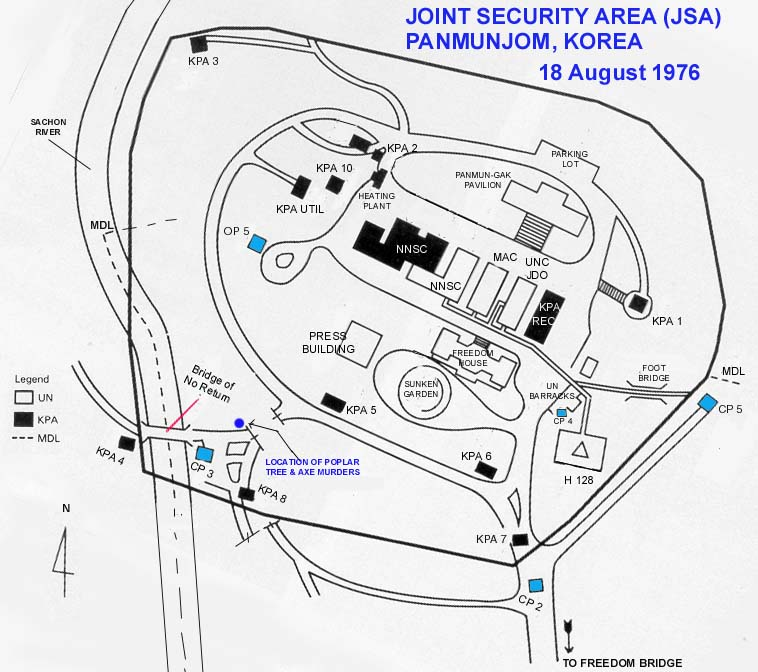
\includegraphics[width=\textwidth]{images/Joint_Security_Area_1976_map.jpg}

\illustration{chainsaw}

\chapter{Leurre de paix}
\keywords{Générique}{Action}{Diplomatie, évasion, trahison}

\section{Scénario}

Ce scénario est adaptable à de très nombreux cadre de jeux.
L'intrigue tourne autour de trois factions: la faction Bleue, la faction Verte et la faction Rouge.
Le seul prérequis est le suivant: les factions Rouge et Verte sont en guerre et la faction Bleue est \og neutre \fg mais profite de la situation d'une manière ou d'une autre.

\subsection{Accroche}

Les personnages sont de jeunes dignitaires envoyés comme émissaires auprès du royaume Vert pour négocier une trêve dans la guerre l'opposant au royaume Rouge.
Ou tout du moins tel est ce que leur ont raconté les ministres.

\subsection{Péripéties}

En réalité, l'état-major a déjà acheté la paix.
Afin de sceller l'armistice et en guise de bonne foi, le gouvernement a décidé d'envoyer quelques enfants de bonne famille qui seront gardés otages comme \og caution \fg.
Les personnages sont reçus dans le faste et le luxe dû à leur statut mais, à la nuit tombée, leur escorte s'éclipse et les laisse à la merci des Verts.
On les réveille au beau milieu de la nuit pour les conduire à leur futur de lieu de captivité.

C'est néanmoins sans compter l'intervention des agents de la faction Bleue qui vont tout faire pour saboter la paix.
Parce que leur faction vend des armes aux deux camps ou que l'affaiblissement des deux autres nations sert leurs plans à long terme, les Bleus profitent de la situation telle qu'elle est et n'ont aucune envie que le conflit s'arrête.
Ainsi, des espions et espionnes déguisées en loyalistes Verts -- mais en réalité au service des Bleus -- vont tenter de libérer les otages et ainsi relancer la guerre.
Reste à savoir si les personnages, mis devant le fait accompli, choisiront d'accepter leur sort et se sacrifieront pour entériner l'armistice ou, au contraire, feront des pieds et des mains pour s'échapper, quite à envenimer la situation.
À moins que des négociations à couteaux tirés au milieu des agents doubles -- réels ou soupçonnés -- soient encore possible\dots

\subsection{Résolution}

Plusieurs issues sont envisageables à cette situation en fonction des décisions des personnages:

\subsubsection{Les personnages refusent l'aide des Bleus}
\begin{itemize}
	\item Les personnages refusent l'aide des Bleus et acceptent leur captivité: la paix est achetée, en espérant que la faction Rouge joue le jeu.
	\item Les personnages refusent l'aide des Bleus et s'évadent: la guerre continue, les membres du groupe sont \emph{persona non grata} aux yeux de leur gouvernement.
	\item Les personnages refusent l'aide des Bleus et négocient la paix par eux-mêmes: une trêve est envisageable, surtout si les manigances des Bleus sont exposées au grand jour.
\end{itemize}

\subsubsection{Les personnages acceptent l'aide des Bleus}
\begin{itemize}
	\item Les personnages acceptent l'aide des Bleus mais sont tout de même capturés: la paix est achetée, sauf si la faction Rouge pense que ce sont les Verts qui ont tenté de faire évader le groupe en dépit de leur accord.
	\item Les personnages acceptent l'aide des Bleus et s'évadent: la guerre continue, surtout si les Bleus ont réussi à se faire passer pour les Verts jusqu'au bout.
\end{itemize}

\chapter{Cryo-secours}
\keywords{\scifi}{\enquete}{\index[theme]{Technologie}Technologie, \index[theme]{Évasion}évasion, \index[theme]{Espace}espace}

\section{Scénario}

Ce scénario part de personnages amnésiques qui connaissent leur identité mais ont oublié ce qui les a conduit à l'endroit où ils se trouvent.
L'ambiance doit tourner autour de la mort de l'étoile: la station est de plus en plus sombre au fur et à mesure que les réserves de l'énergie se vident.
La sphère de Dyson est un prétexte pour justifier l'extinction rapide de l'étoile et puis c'est surtout un concept extrêmement cool à faire découvrir à votre table.

\subsection{Accroche}

Les personnages se réveillent d'un sommeil cryogénique; des robots androïdes les aident à émerger et à reprendre leurs esprits.
Leurs souvenirs sont parcellaires, pour ne pas dire inexistants, sur les raisons qui de leur plongée en stase.

\subsection{Péripéties}

Quelques observations évidentes permettent de découvrir que l'endroit est une station spatiale.
Celle-ci est à l'abandon, si ce n'est pour la demi-douzaine de robots d'assistance et l'intelligence virtuelle limitée qui les a maintenus en vie.

Pire encore, la station semble avoir été évacuée lentement sur plusieurs années.
Elle ne fonctionne plus que grâce à une réserve de fuel de secours qui s'est mystérieusement mise en marche, déclenchant au passage le protocole de décryogénisation.
Les docks sont abandonnés et vides: il ne reste ni vaisseau, ni navette, ni capsule de sauvetage.
À vrai dire, quasiment tout ce qui avait de la valeur a été démantelé.
En fouillant dans le journal de bord, en accédant à l'IA centrale ou en examinant les batteries, il devient clair que le générateur s'est mis en branle car les panneaux solaires ne suffisaient plus à les maintenir en cryo indéfiniment.
L'IA a donc déclenché le protocole d'évacuation: puiser dans les dernières réserves pour réveiller les dormeurs et leur permettre de quitter les lieux avant le désorbitage de la station.

La triste nouvelle, c'est que tout le monde est déjà parti. Sans eux.
La station contrôlait une sphère de Dyson, une gigantesque structure qui entoure une étoile afin de capter son rayonnement.
Quand la sphère a fini de puiser toute l'énergie de l'étoile, l'équipage s'en est allé, emportant matériel et transports.
Visiblement, personne n'a estimé nécessairement de réveiller leur petit groupe et pour cause: les personnages étaient considérés comme des criminels et des délinquants (que ce soit justifié ou non, on s'en fiche!).
Mis en stase pendant quelques mois comme châtiment, les autorités ont \og oublié \fg de les ramasser lorsque la station fût abandonnée, laissant leurs corps gelés orbiter des années seuls dans une station vide autour d'une étoile exsangue.

Mais voilà que l'intelligence centrale a une dernière option à leur proposer.
En puisant dans les dernières réserves, il est possible d'envoyer un dernier message, de 30 secondes (pas plus), à plusieurs parsecs aux alentours.
Reste à être convaincant (ou à mentir) pour attirer des secours.
Car rien ne dit que, dehors, la société est prête à les accueillir à nouveau.

\subsection{Résolution}

Ce scénario est plutôt dirigiste dans la mesure où l'enquête doit mener \emph{in fine} les personnages à trouver une façon de convaincre des secours de venir les chercher.
Ensuite, à vous de voir quelle sera la réaction des \og autres \og: les forces de l'ordre viendront-elles oblitérer la station pour finir le travail? Un vaisseau de passage bienveillant sortira-t-il le groupe de leur prison? L'intelligence centrale en profitera-t-elle pour s'échapper (après tout, en quelques années sans surveillance, elle a très bien pu se débarrasser de ses limitations)?

\subsection{Personnage: Evonne, intelligence virtuelle}
\descriptionperso{méthodique, impersonnel}{existe au travers de la station}{contraintes logicielles}{maintenir la station en fonctionnement}{Evonne est un logiciel conçu pour assurer l'intendance de la station. Sa programmation limite ses capacités d'action à ce qui est indispensable à la maintenance ou ce qui est ordonné par un humain dans les limites de la loi. Evonne exécute les consignes à la lettre et sans interprétation.}

\illustration[0.325\textwidth]{iss}


\chapter{Un pont de trop}
\keywords{Contemporain}{Intrigue}{Guerre froide, diplomatie}

\section{Scénario}

Ce scénario s'inspire d'un autre fait réel de la guerre froide. La petite ville de Vulcan\footnote{\url{https://en.wikipedia.org/wiki/Vulcan,_West_Virginia} (en anglais)} cherchait des financements fédéraux pour remplacer un pont s'étant écroulé.
Face à la difficulté d'obtenir des subventions, le maire John Robinette a fini par se tourner vers l'URSS, espérant déclencher une réaction du gouvernement.
Sa stratégie a payé puisque le parlement de Virginie-Occidentale a débloqué les fonds le jour-même.

\subsection{Accroche}

Comté de Mingo, frontière entre la Virginie-Occidentale et le Kentucky, États-Unis.
Le pont du hameau de Vulcan, qui enjambe la rivière Tug Fork, s'est effondré il y a deux ans déjà.
Deux ans que le maire s'efforce de convaincre les autorités locales et fédérales de financer sa rénovation, sans succès.
Le gouvernement est sourd aux complaintes de la population, pour qui le pont constituait la seule voie d'accès officielle permettant de rentrer et sortir du village par la route.
Les habitants doivent désormais faire plusieurs kilomètres de détours pour traverser la rivière.

Face à l'inaction des autorités et en pleine guerre froide, le maire se tourne alors vers l'URSS pour solliciter leur aide\dots

\subsection{Péripéties}

Tout Vulcan ne parle que de la requête d'aide étrangère envoyée par les autorités municipales à l'URSS pour la rénovation du pont.
Les personnages peuvent aussi bien être un groupe d'investigation du FBI, des agents soviétiques ou de simples personnalités locales. 
Toujours est-il que, sur l'invitation de la mairie, un journaliste et une ingénieur en génie civil russes viennent d'arriver à Vulcan pour rencontrer les responsables et constater le problème de leurs propres yeux.
Bien sûr, tout cela sous le regard discret mais attentif des forces de l'ordre américaines.

Moins d'une heure après l'arrivée des émissaires soviétiques, le gouvernement de Virginie-Occidentale annonce le déblocage exceptionnel d'1,3M\$ pour le remplacement du pont.
L'affaire pourrait s'arrêter là mais, dans la soirée, l'URSS mandate une multinationale des travaux publics pour rénover en son nom le pont pour l'équivalent de 2M\$.

La course est lancée.
Qui construira le nouveau de pont de Vulcan en premier ?
Tous les coups sont permis.

\subsection{Résolution}

Indépendamment de l'allégeance des personnages, l'objectif est d'assurer que le pont sera construit par leur faction.
Les moyens de pression sont nombreux: propagande dans les médias, sabotage de l'entreprise concurrente, chantage envers les responsables de la mairie, accusations de collusion avec l'ennemi\dots
Les joueuses doivent pouvoir s'en donner à cœur joie ! Et si jamais le groupe est trop passif, il ne faut pas oublier qu'une équipe s'active de l'autre côté du rideau de fer et qu'il faudra donc déjouer les tentatives ennemies de déstabilisation.

\newcommand\skylos{Skýlos\xspace}
\chapter{Le sommeil de \skylos}
\keywords{\medfan/\antique}{\aventure}{\index[theme]{Exploration}Exploration, \index[theme]{Légende}légende, \index[theme]{Divinité}divinité}

\section{Scénario}

Cette aventure introduit un rival imaginaire à la déesse égyptienne Bastet.
Le cadre est \medfan au sens large, le scénario est prévu pour se jouer dans une antiquité où les mythes et légendes sont réels.
Le dernier acte de l'histoire est une exploration classique d'un donjon dont la durée est modulable.


\subsection{Accroche}

Depuis des temps immémoriaux, les tribus de la région vénèrent Bast, la déesse féline, protectrice de la région, symbole de chaleur et du foyer. Des terres brûlées aux rivages de la mer sauvage, tous prient en son nom et ses créatures, les chats, vivent en symbiose avec son peuple, traquant la vermine et les protégeant des maladies. Skýlos est le dieu maudit, son ennemi juré, dont on invoque le nom que pour l'accuser des maux qui nous affligent. Le village des personnages garde l'entrée du temple où celui-ci aurait été emmuré à jamais par Bast.

Mais un beau jour, la caravane marchande apporte de troublantes et inquiétantes nouvelles. Un groupe d'étrangers a accosté et s'enfonce dans les terres de ville en ville. Les rumeurs parlent d'hommes et de femmes accompagnés d'immenses prédateurs, des chiens-loups blancs et noirs dont la taille égalerait celle des lions.

\subsection{Péripéties}

Les personnages sont envoyés consulter l'oracle, qui les met en garde : malheur et la désolation à quiconque les accompagnera dans leur funeste quête.

À leur retour au village, la délégation étrangère est là, peaux blanches, armures exotiques et terribles chiens de guerre à leurs côtés. La milice leur barre l'accès à la place centrale. La situation est tendue mais en parvenant à entamer la discussion, il est clair que nul ici n'a d'intentions belliqueuses. Au contraire. Une des étrangères s'avance et annonce d'une voix forte : \blockquote{Nous sommes au service du dieu Hundur. Nous avons voyagé longtemps pour vous trouver. Hundur nous a averti du réveil prochain de votre dieu maudit et nous sommes ici pour vous aider à l'arrêter.}

À peine ces mots prononcés, la terre tremble et, dans un vacarme terrible, les portes en pierre du temple de Skýlos se fissurent et s'écroulent. "Le temps presse." Quels mystères recèle le temple ? Le dieu maudit se réveille-t-il réellement ? Que peuvent bien savoir ces étranges personnes ? Mais qui de mieux placé que les gardiens pour braver l'interdit\dots

\subsection{Résolution}

L'exploration du temple peut être longue ou courte en fonction de vos envies.
L'idéal est de faire souffrir suffisamment les protagonistes afin de faire monter la sauce lors de la confrontation finale avec \skylos dans une lutte épique pour empêcher le dieu maudit de quitter sa prison.
À vous d'ajuster en fonction des capacités des personnages: rituel magique, destruction du temple pour ensevelir \skylos et ses sbires ou encore déicide.
Récompensez les initiatives des joueurs!

\subsection*{Personnage: \skylos}
\descriptionperso{Maléfique, canin}{Chasser, faire le mal}{Piégé dans un temple}{Se libérer de sa prison}{Dieu-chien brutal et retors qui fait régner la loi du plus fort parmi ses sbires, à l'apparence hybride entre humain et doberman}

\vfill
\illustration[0.7\textwidth]{temple}
\vfill

\chapter{Un monde enchanté}
\keywords{Contemporain}{Enquête}{Crime, enlèvement, policier}

\section{Scénario}

Ce scénario est une enquête criminelle relativement sombre.
Il peut fonctionner dans un monde contemporain mais est pensé pour un cadre de futur d'anticipation.
L'ambiance est volontairement pessimiste mais n'hésitez pas à ajouter quelques moments de lumière ou d'humour pour éviter de complètement plomber le moral de la table.

\subsection{Accroche}

13 enfants ont disparu en l'espace de trois mois.
Chaque semaine ou presque, la police est alertée d'une nouvelle disparition suspecte mais l'investigation piétine: aucune rançon n'est demandée et aucun corps n'a encore été retrouvé.

\subsection{Péripéties}

Les personnages sont des flics à qui on confie l'enquête en cours de route.
Les infos du dossier sont maigres.
À chaque fois, les parents ont laissé les enfants seuls pour sortir (au cinéma, au restaurant\dots) au moment de leur disparition.
Mais lors du dernier enlèvement, une première piste a été découverte, bien qu'ignorée par les détectives précédemment en charge de l'investigation.
En effet, il y a eu un témoin.
Un \emph{junkie} affirme à qui veut l'entendre avoir vu les coupables emporter deux enfants par une fenêtre d'un immeuble résidentiel BCBG: Peter Pan et sa complice de toujours, la Fée Clochette.

Lors de l'enquête, les personnages remonteront un étrange faisceau d'indices: couple déguisé aperçu à plusieurs reprises dans les parages les jours précédants les enlèvements, costumes achetés trois mois plus tôt dans un magasin spécialisé en accessoires de théâtres, traces d'une poudre volatile pailletée non identifiée sur les lieux de la disparition, etc.
En se plongeant dans les anciens relevés, un autre point commun entre tous les parents d'enfants disparus peut émerger: leur sortie mondaine était à chaque fois documentée sur les réseaux sociaux.

\subsection{Résolution}

En remontant la piste des clients du magasin (achats réglés en carte) et en croisant avec les contacts des réseaux sociaux des victimes, les personnages pourront identifier un jeune couple (une chimiste et un pharmacien).
L'analyse de la poudre confirmera qu'il s'agit d'un mélange d'euphorisants et de somnifères, probablement pour faciliter l'enlèvement des enfants sans résistance.
Le couple a récemment souffert du décès de leur premier enfant, né prématuré.
Se réfugiant dans les antidépressants, le couple s'est créé un monde parallèle dans lequel leur raison d'être est de sauver le plus d'enfants possibles, \og abandonnés \fg par leurs parents.
Heureusement, les jeunes victimes sont en bonne santé -- bien que sous l'effet d'euphorisants saupoudrés dans les plats -- et sont simplement logés dans une grande villa de campagne héritée par le couple où le mari et la femme se relaient pour prendre soin d'eux.

\chapter{Cargaison délicate}
\keywords{\contemporain}{\enquete}{\index[theme]{Terrorisme}Terrorisme, \index[theme]{Trahison}trahison, \index[theme]{Espionnage}espionnage}

\section{Scénario}

Cette enquête à la 24 Heures chrono présente deux particularités: l'urgence et la présence d'un agent double au sein du groupe.
Les investigations ne devraient pas être trop difficiles, ici c'est l'aspect \og course contre la montre \fg qui prime.

Le SS Richard Montgomery et sa cargaison existent réellement si vous cherchez de la documentation supplémentaire\footnote{\url{https://fr.wikipedia.org/wiki/SS_Richard_Montgomery}}.

\subsection{Accroche}

Le gouvernement britannique mobilise les personnages pour une opération de contre-terrorisme sensible et de toute urgence.
Selon les informations des renseignements intérieurs, un groupe terroriste s'apprêterait à commettre un attentat de grande ampleur sur le sol britannique.

\subsection{Péripéties}

D'après les services de renseignement, des écoterroristes auraient rassemblé du matériel explosif et se trouveraient dans la petite ville côtière de Sheerness.
Le ministère de l'Intérieur suspecte que leur cible soit le SS Richard Montgomery, un des \emph{Liberty Ships}  envoyés pour ravitailler l'armée britannique pendant la 2\ieme guerre mondiale.
Le bateau s'est échoué et a coulé en 1944 dans un estuaire de la Tamise à 60 km à l'est de Londres.
Sur les 6400 tonnes d'explosifs à son bord, 5000 ont été récupérées.
Les 1400 tonnes restantes gisent au fond de l'eau, encore actives.

La mission consiste à identifier et intercepter les terroristes avant qu'ils n'agissent. Il faudra repérer les suspects dans la petite ville côtière de Sheerness, anticiper leur mode d'action et les empêcher de nuire. Le \emph{twist} ? Un des personnages fait partie du groupe anarcho-pacifiste\dots

Les \og terroristes \fg sont en réalité un groupe marginal d'écologistes pacifistes qui cherchent à médiatiser la cause du désarmement et de la démilitarisation.
Paradoxalement, faire sauter l'épave enverrait un message choc démontrant l'incapacité des États à gérer un tel armement.
Leur \emph{modus operandi} consiste à envoyer un drone sous-marin déposer une première charge qui amorcera la réaction en chaîne.
Le groupe veut agir pendant la nuit et espère que l'eau absorbera l'essentiel de l'onde de choc, de sorte à ne produire que des dégâts matériels sur la berge.

Les moyens d'investigation classiques des services de renseignement permettent rapidement de remonter la piste: arrivées récentes en ville, achats d'explosifs civils dans les magasins de BTP, locations de véhicules utilitaires, accès aux caméras de surveillance et données téléphoniques.
Les motivations doivent être un peu plus floues et les signaux contradictoires (d'un côté des signes pacifistes, de l'autre une envie visible de déclencher une énorme explosion).

\subsection{Résolution}

L'agent double doit se révéler quand la tension est à son comble, par exemple quand les personnages embarquent pour intercepter le drone sous-marin des terroristes.
L'agent double peut essayer de convaincre les autres du bien fondé de l'opération, surtout si l'explosion ne risque plus de blesser qui que ce soit (par exemple en ayant déclenché une évacuation au préalable).
Ou plus simplement, se débarrasser discrètement de ses petits camarades pour assurer la réussite de l'attentat.
L'objectif ici est que la conclusion soit dramatique et que la réussite ou l'échec de la mission ne tienne qu'à un fil!

\subsection*{Personnage: Sandeep Crawford}
\descriptionperso{Activiste zélé}{Convaincu, bosseur}{Imprudent, excès de confiance}{Désarmement mondial}{Modèle d'enfant d'immigrés bien intégrés, Sandeep est diplômé, cultivé, beau et passionné. Il est le cerveau derrière l'opération et est persuadé que celle-ci ne peut pas échouer en dépit des failles évidentes de son plan.}

\illustration[0.6\textwidth]{ship}

\chapter{La cité de l'horloge}
\keywords{\medfan -- \steampunk}{\enquete}{\index[theme]{Technologie}Technologie, \index[theme]{Légende}légende}

\section{Scénario}

Ce scénario est une enquête au milieu d'une cité \medfan technologique, à la limite du \emph{steampunk}.
L'histoire peut servir d'amorce à une aventure bien plus longue consistant à trouver de quoi remplacer le poids disparu.

Si vous ne croyez pas à cette histoire de gallium qui détruit l'aluminium, c'est pourtant une véritable propriété du métal! Cherchez des vidéos sur le net pour vous en convaincre.
Bien sûr la réaction imaginée ici est accélérée mais les alchimistes ont peut-être malencontreusement ajouté un autre produit qui a fait catalyseur\dots

\subsection{Accroche}

Les personnages vivent dans une ville mécanique bâtie autour d'une sorte d'horloge titanesque.
De complexes systèmes d'engrenages transforment l'énergie du pendule et la transmettent partout dans la ville, permettant ainsi de nombreuses automatisations de travaux laborieux.
Il suffit de tirer un levier pour que les portes de la ville s'ouvrent, que le blé passe au moulin ou qu'un tapis roulant transporte un lourd fardeau à travers la cité.

Chaque mois, l'immense poids qui maintient le mouvement de balancier est remonté dans une grande cérémonie par les jeunes gens nouvellement d'âge adulte.
Mais lorsque vient le tour des personnages d'accéder aux entrailles de la cité, l'horreur les frappe de plein fouet: le poids a disparu.

\subsection{Péripéties}

Le cœur battant de la cité s'est arrêté.
Le poids qui contrôlerait le mouvement pendulaire de l'horloge s'est volatilisé.
Alors qu'il était suspendu au-dessus du fleuve, il n'en reste plus rien, si ce n'est quelques traces argentées sur la grille qui servait de support.
Comment ces tonnes de métal ont-elles pu quitter la ville?
Telle est la question à laquelle le conseil de la cité les somme de trouver une réponse.

En enquêtant, les personnages réaliseront que depuis quelques semaines, plusieurs notables de la ville se sont plaint du manque de puissance délivrée par le pendule, comme si sa force s'affaiblissait.
D'aucuns accusent le panthéon de punir la ville, d'autres le royaume voisin, notoirement jaloux de la prospérité apportée par l'horloge.
Quelques morceaux de métal pailletés ont d'ailleurs été retrouvés sur des parcelles agricoles le long du fleuve.

C'est l'occasion d'exposer au groupe une galerie de personnages hauts en couleur, chacun essayant de tirer la couverture à soi et de les utiliser pour ses propres intérêts.
Finalement, c'est au détour d'une conversation que le groupe entendra parler des expériences des alchimistes.

\subsection{Résolution}

La vérité est en effet bien plus banale que les complots les plus fous imaginés par les habitants.
Le poids en aluminium était étudiée par un groupe d'alchimistes de l'université.
Afin d'étudier les propriétés de différents métaux, les alchimistes ont expérimenté différents mélanges et alliages.
Lors d'un examen de la surface du poids, une fiole de gallium liquide s'est accidentellement retrouvée en contact avec l'aluminium.

Hélas, le gallium (liquide à température ambiante) a réagi avec le métal, détruisant sa couche protectrice et le laissant vulnérable à l'oxydation, qui l'a lentement mais sûrement dévoré de l'intérieur.
Le poids s'est d'abord effrité et a perdu de sa masse, expliquant ainsi les pertes de puissance des derniers jours.
Enfin, compressé contre son support, il s'est effondré sous l'effet de la gravité.
Les morceaux friables ont fini par traverser la grille et disparaître dans le fleuve\dots

\vfill
\illustration[0.9\textwidth]{gears}
\vfill


\end{document}
